\documentclass[11pt,a4paper,oneside]{book}

\usepackage[T1]{fontenc}
\usepackage[utf8]{inputenc}
\usepackage[czech,english]{babel}

\usepackage{amsmath}
\usepackage{amssymb}
\usepackage{amsthm}

\usepackage{newtxtext}
\usepackage{newtxmath}

\usepackage[
  a4paper,
  tmargin=4cm,
  bmargin=3cm,
  lmargin=3cm,
  rmargin=2cm,
  headheight=0.8cm,
  headsep=1cm,
  footskip=0.5cm
]{geometry}

\usepackage{graphicx}
\usepackage{pdfpages}
\usepackage{setspace}
\usepackage{indentfirst}
\usepackage{microtype}
\usepackage{booktabs}
\usepackage{enumitem}
\usepackage{url}

\usepackage[
  colorlinks=true,
  linkcolor=black,
  citecolor=black,
  filecolor=black,
  urlcolor=blue
]{hyperref}

% --- Bibliography Setup ---
\usepackage[
  backend=biber,
  style=numeric,
  sorting=none,
  giveninits=true,
  maxbibnames=99
]{biblatex}

\addbibresource{Bibliography.bib}

\setlength{\bibitemsep}{1em}

\clubpenalty=9500
\widowpenalty=9500

\renewcommand{\vec}[1]{\boldsymbol{#1}}

\newcommand{\CZ}{\selectlanguage{czech}}
\newcommand{\EN}{\selectlanguage{english}}

\newcommand{\documentdate}{June 20, 2026}

\begin{document}

% -------- FRONT MATTER --------
\frontmatter
\pagestyle{empty}

\begin{titlepage}
\centering

\begin{minipage}[c]{3cm}
\centering

\includegraphics[width=3cm]{Images/TITLE/cvut}
\end{minipage}
\hfill
\begin{minipage}[c]{0.6\linewidth}
\centering
{\large\textsc{Czech Technical University in Prague}}\\
{\large Faculty of Nuclear Sciences and Physical Engineering}
\end{minipage}
\hfill
\begin{minipage}[c]{3cm}
\centering

\includegraphics[width=3cm]{Images/TITLE/fjfi}
\end{minipage}

\vspace{3cm}

{\huge\bfseries Automatic Monitoring of Data Drift and Model Performance\par}
\vspace{1cm}

\CZ
{\huge\bfseries Automatický monitoring driftu dat a výkonu modelu\par}
\EN

\vspace{2cm}
{\large Bachelor's Degree Project\par}

\vfill

\begin{tabular}{@{}ll@{}}
Author: & \textbf{Bexultan Zhaskairat}\\
Supervisor: & \textbf{RNDr. Zuzana Petříčková, Ph.D.}\\
Consultant: & \textbf{doc. RNDr. Jméno Konzultanta, CSc.} \\
Academic year: & 2025/2026\\
\end{tabular}

\vspace{1cm}
{\large \documentdate\par}

\end{titlepage}


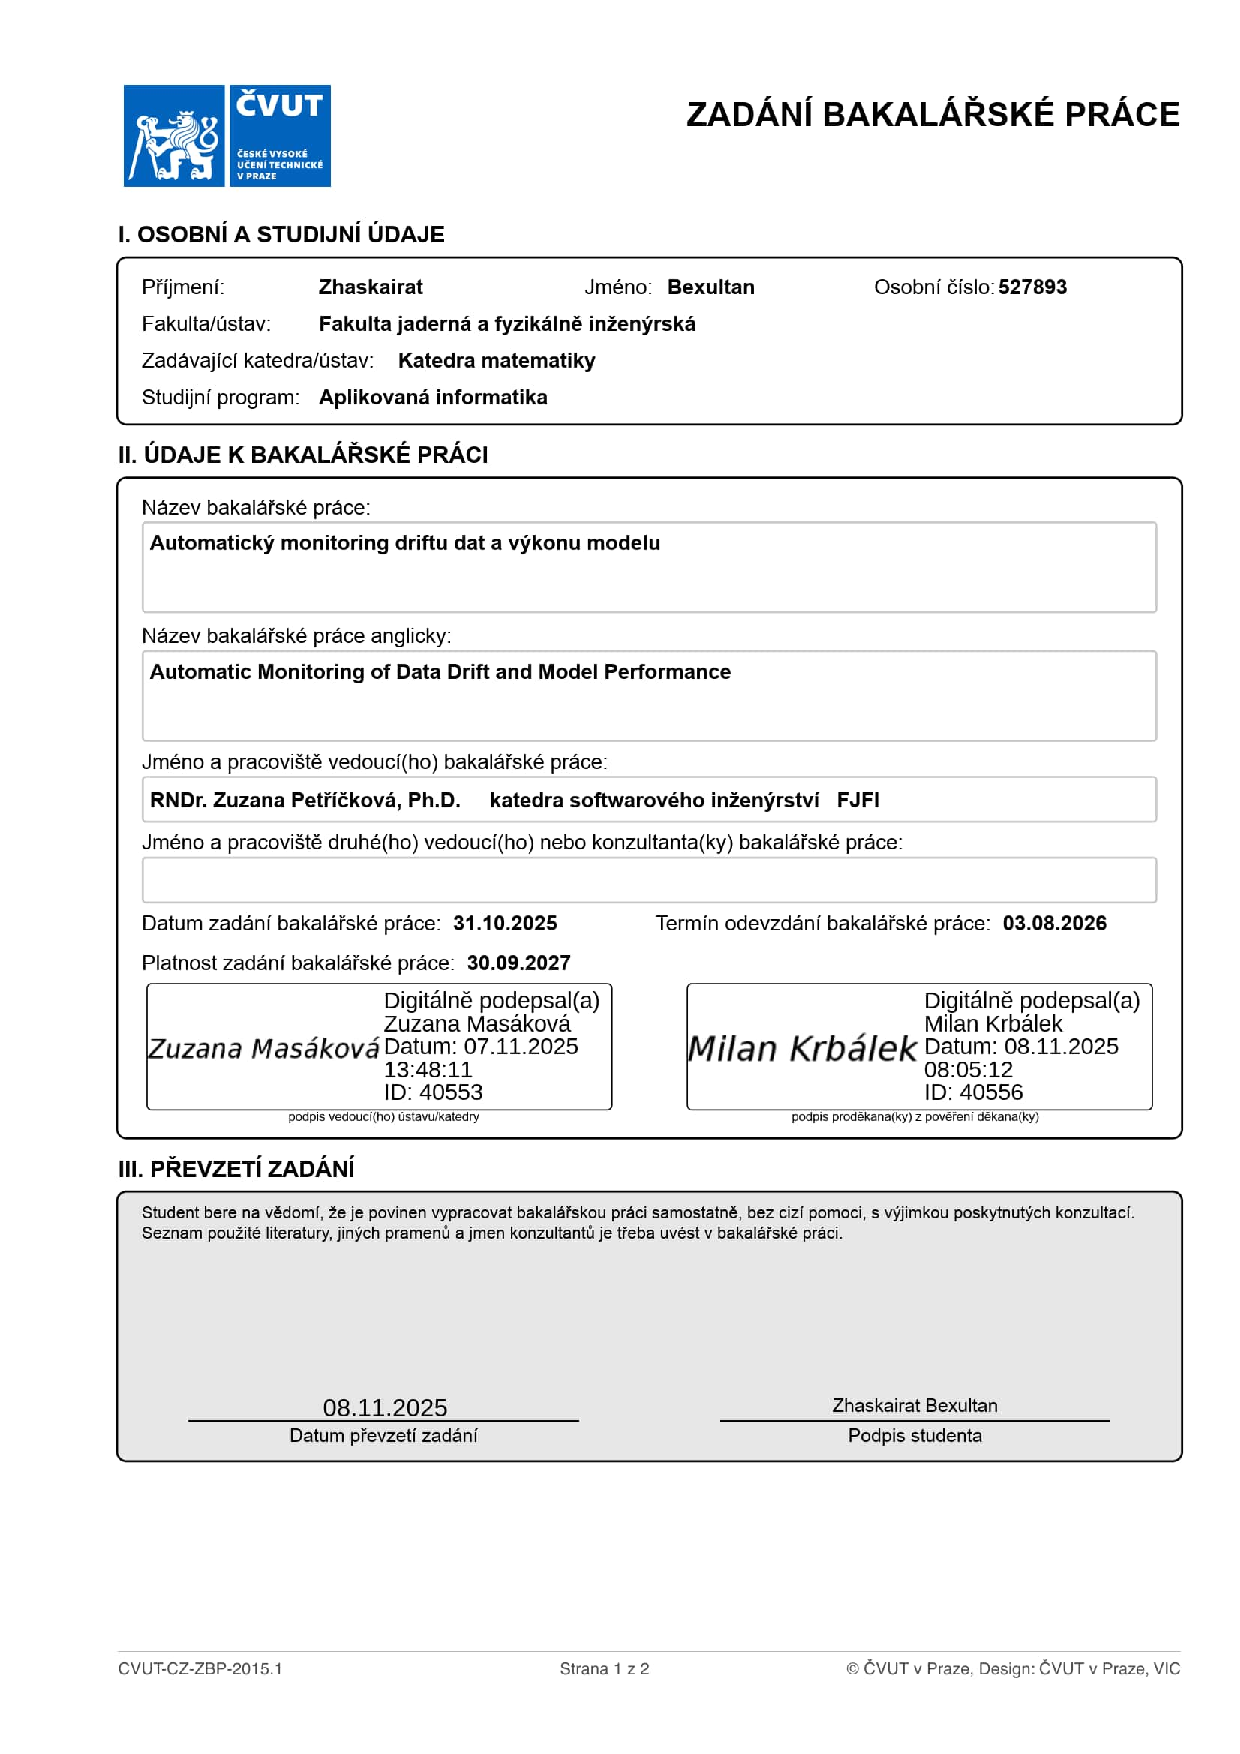
\includepdf[pages=-]{pdf/zadani_bk.pdf}
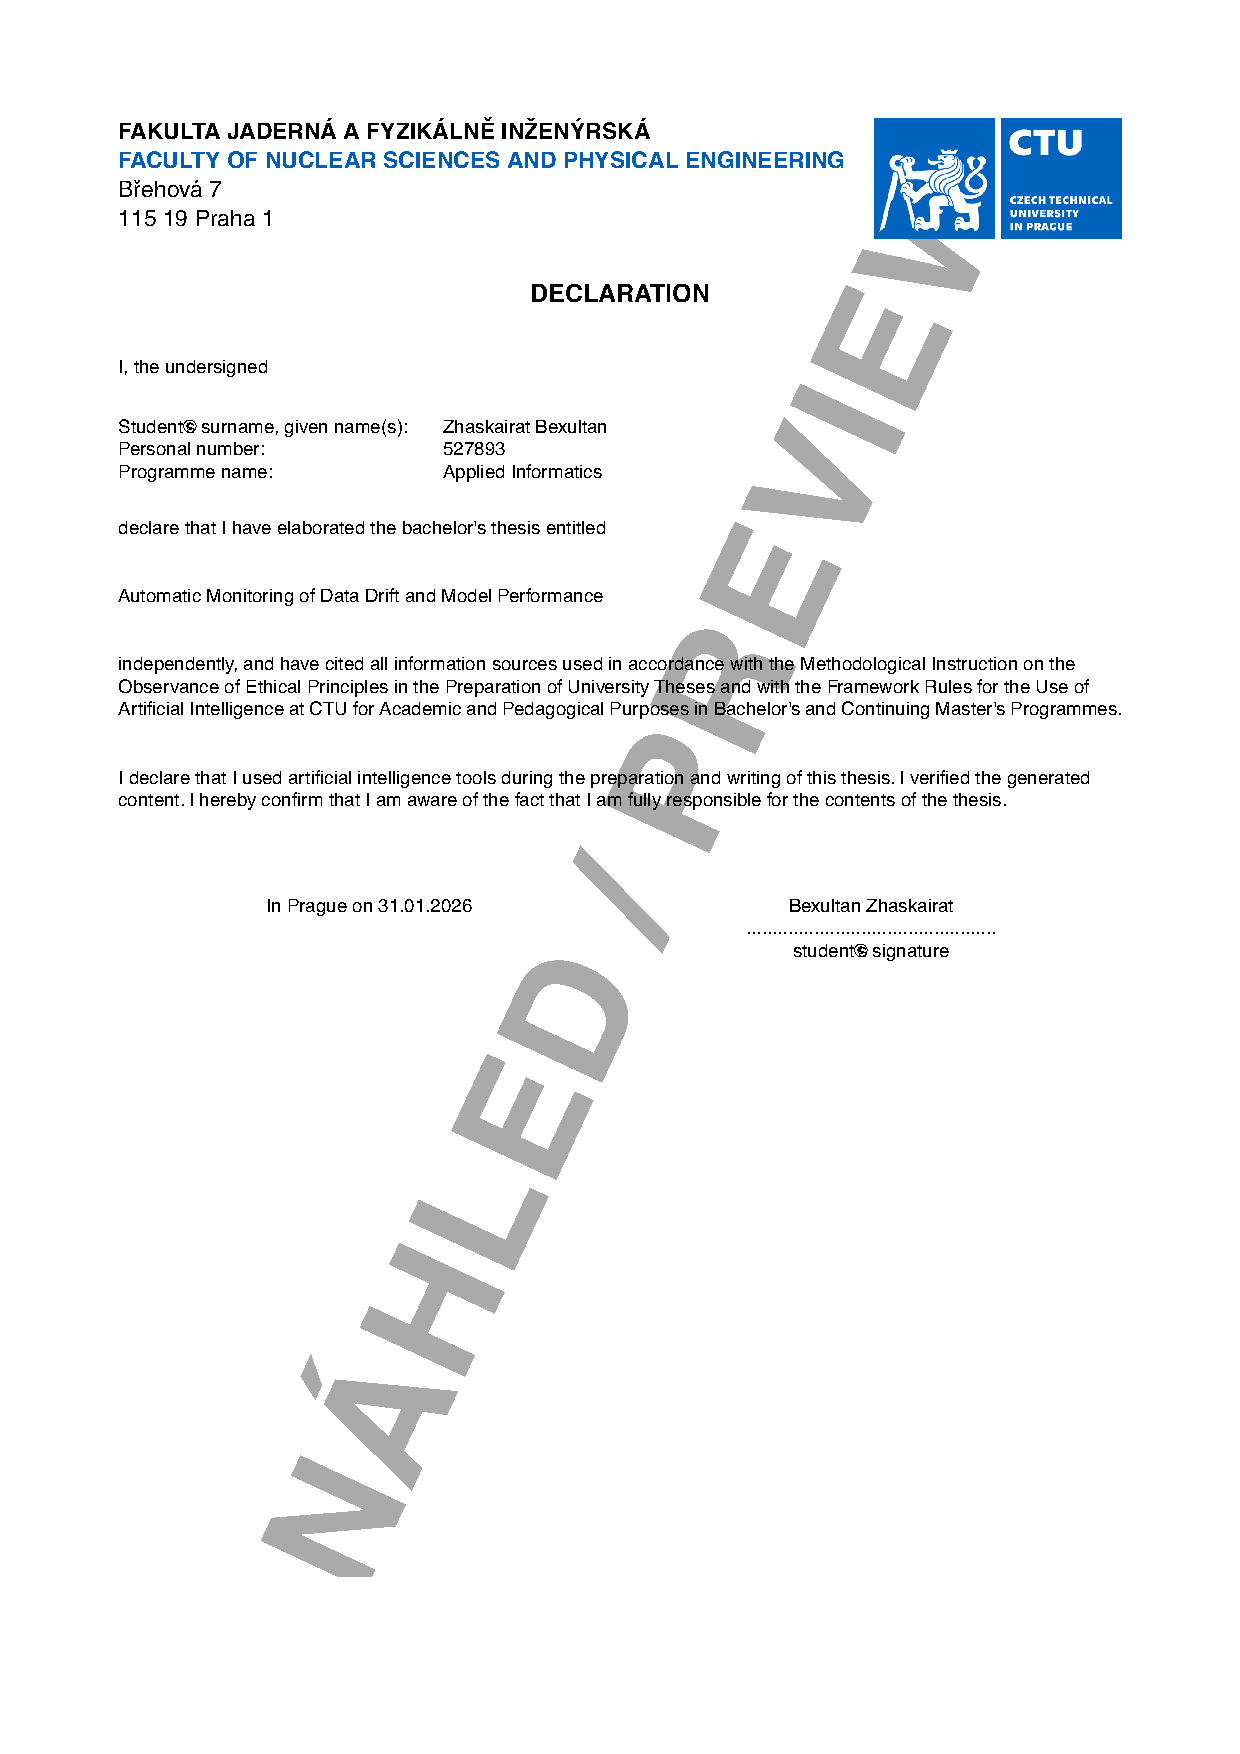
\includepdf[pages=-]{pdf/prohlaseni.pdf}

\pagestyle{empty}
\noindent{\Large\emph{ Acknowledgments:}}\par
\vspace{0.5cm}

\noindent
I would like to thank \dots\ for \dots\ and express my gratitude to \dots\ for \dots

\vspace{1cm}
\begin{flushright}
\textbf{Bexultan Zhaskairat}
\end{flushright}

\clearpage

\CZ
\begin{onehalfspace}
\noindent\emph{Název práce:}\\
\textbf{Automatický monitoring driftu dat a výkonu modelu}

\bigskip
\noindent\emph{Autor:} Bexultan Zhaskairat

\bigskip
\noindent\emph{Studijní program:} Aplikovaná informatika

\bigskip
\noindent\emph{Druh práce:} Bakalářská práce

\bigskip
\noindent\emph{Vedoucí práce:} RNDr. Zuzana Petříčková, Ph.D.

\bigskip
\noindent\emph{Abstrakt:}\\
% TODO: текст

\bigskip
\noindent\emph{Klíčová slova:}
automatický monitoring, concept drift, data drift, detekce anomálií, MLOps, produkční systémy, strojové učení, výkonnost modelu.
\end{onehalfspace}
\EN

\clearpage

\EN
\begin{onehalfspace}
\noindent\emph{Title:}\\
\textbf{Automatic Monitoring of Data Drift and Model Performance}

\bigskip
\noindent\emph{Author:} Bexultan Zhaskairat

\bigskip
\noindent\emph{Abstract:}\\
% TODO: text

\bigskip
\noindent\emph{Key words:}
anomaly detection, concept drift, data drift, machine learning, MLOps, model monitoring, model performance, production systems.
\end{onehalfspace}

\clearpage

% -------- MAIN MATTER --------
\mainmatter
\pagestyle{headings}

\pagenumbering{arabic}
\setcounter{page}{8}

\tableofcontents
\clearpage

\chapter*{Introduction}
\addcontentsline{toc}{chapter}{Introduction}

Machine learning models are widely used in real-world applications to support decision-making and automate business processes. However, their performance can decrease after deployment because production data may change over time due to shifts in user behavior, external conditions, business processes, missing data, application errors, schema changes, or changes in data sources \cite{MonitoringPerformance,MachineLearningModelinProduction}. This problem is closely related to data drift, where the data used in production becomes different from the data used during training or validation \cite{MonitoringPerformance}.

Because of this, model monitoring is an important part of the machine learning lifecycle. It helps observe whether a deployed model continues to behave as expected in production. Monitoring can include tracking prediction quality, error rates, confidence scores, latency, feature distributions, missing values, and schema changes \cite{MonitoringPerformance}.

A reliable monitoring process should also focus on input data quality. Important indicators include data volume, average values of input variables, and missing or null values \cite{MonitoringPerformance}. In addition, statistical methods such as Population Stability Index, Kolmogorov--Smirnov test, Wasserstein distance, and Chi-square test can be used to compare reference data with current data \cite{EvidentlyDataDriftLargeDatasets,SciPyDocumentation}. If significant differences are detected, alerts can notify developers or data scientists that the model may no longer be performing reliably.

The aim of this bachelor thesis is to design and implement a prototype system for automatic monitoring of data drift and model performance. The project focuses on operational monitoring of machine learning models, data quality checks, batch and streaming drift detection, model performance evaluation, result storage, and dashboard visualization.

\clearpage

% -------- CHAPTERS --------
\chapter{Operational Monitoring of Machine Learning Models}
\label{ch:operational-monitoring}

\section{Machine Learning Models in Production}

Machine learning models are usually trained on historical data and later applied to new data in a production environment. In contrast to traditional software, the behavior of an ML model depends not only on source code, but also on the statistical properties of the data used during inference. Therefore, a deployed model can become less reliable even when the application code remains unchanged.

Production model performance can degrade because of changes in the external environment, missing input features, schema changes, data quality problems, seasonality, or changes in user behavior \cite{MonitoringPerformance}. This means that a model which performed well during training and validation may later produce weaker predictions on current production data.

For this reason, monitoring is an important part of the MLOps lifecycle. ML implementation is commonly described as an end-to-end process that includes data handling, model building, validation, deployment, continuous monitoring, performance tracking, and maintenance \cite{MachineLearningModelinProduction}. In this thesis, the focus is not placed on building a complete industrial MLOps platform, but on implementing the monitoring part of this lifecycle.

A production ML system should therefore be observed not only as software, but also as a data-driven decision system. Traditional monitoring can detect technical failures such as latency or service errors, while ML monitoring must also detect changes in data, predictions, model performance, and business impact \cite{MonitoringObservabilityMLSystems}.

\section{Data Quality and ML-Specific Monitoring}

Standard software monitoring usually focuses on technical indicators such as uptime, latency, memory usage, error rates, or resource consumption. These indicators are important, but they do not show whether an ML model still produces reliable predictions. ML-specific monitoring extends this view by observing the quality of input data, the distribution of model predictions, and the predictive performance of the model.

Data quality is important because poor input data can strongly affect model behavior. Production data may contain missing values, outliers, inconsistent records, different data formats, or changed schemas. These problems can appear because of application bugs, upstream pipeline changes, source system errors, or changes in business processes \cite{MonitoringPerformance}. For this reason, data validation and data quality checks are necessary before drift detection and performance monitoring are interpreted.

A practical ML monitoring process can include checks such as data volume, missing value rate, feature ranges, average feature values, type consistency, and schema compatibility \cite{MonitoringPerformance}. These checks do not directly prove that a model performs poorly, but they can reveal problems that may cause unreliable predictions.

In this thesis, ML-specific monitoring consists of three main parts:

\begin{itemize}
    \item \textbf{Data quality monitoring:} checking whether uploaded datasets have a usable and comparable structure.
    \item \textbf{Data drift monitoring:} comparing feature distributions between reference and current datasets.
    \item \textbf{Model performance monitoring:} evaluating prediction quality when a model and labeled data are available.
\end{itemize}

This separation is useful because each type of monitoring answers a different question. Data quality monitoring checks whether the data is valid. Drift monitoring checks whether the current data is different from the reference data. Performance monitoring checks whether the model still produces acceptable predictions.

\section{Model Performance Degradation and Calibration}

Model performance degradation means that the predictive quality of a deployed model becomes worse over time. This can happen when input data changes, when the relationship between features and the target changes, or when data quality problems appear in the production pipeline \cite{MonitoringPerformance}. A performance drop can lead to incorrect predictions and poor decisions, especially when the model is used in business-critical processes.

Performance degradation can be measured directly only when true labels are available. For classification tasks, common metrics include accuracy, precision, recall, F1-score, and AUC-ROC. For regression tasks, metrics such as MAE, MSE, RMSE, and MAPE can be used \cite{ModelMonitoringFrameworks}. The selected metric must match the goal of the model. For example, recall may be more important in fraud detection, while precision may be more important when false alarms are costly.

Model calibration is also relevant for classification models that output probabilities. A model is well calibrated when predicted probabilities correspond to real outcome frequencies. For example, if a model predicts a probability of 0.8 for a group of cases, approximately 80\% of those cases should belong to the positive class. Poor calibration can make a model unreliable even when its classification accuracy appears acceptable. Calibration can be evaluated using reliability diagrams, which compare predicted confidence with observed accuracy, and by metrics such as Expected Calibration Error (ECE), which calculates the weighted difference between average confidence and average accuracy across confidence bins \cite{UnderstandingModelCalibration}.

In this thesis, calibration is treated as part of the theoretical background. The prototype mainly focuses on drift detection and model performance metrics. However, calibration can be considered as a future extension, especially for classification models where probability outputs are used for decision-making.

\section{Monitoring Indicators: SLA, SLO, and SLI}

Monitoring results must be converted into clear and understandable indicators. In operational systems, this is often described through service-level concepts: SLA, SLO, and SLI.

A \textbf{Service Level Indicator} (SLI) is a measurable value that describes the behavior of a system. In ML monitoring, examples of SLIs include missing value rate, number of drifted features, PSI value, prediction distribution shift, accuracy, F1-score, MAE, or inference latency.

A \textbf{Service Level Objective} (SLO) defines the expected or acceptable level for an indicator. For example, an SLO can state that model accuracy should remain above a selected threshold, that the percentage of missing values should stay below a defined limit, or that PSI should not exceed a selected drift threshold.

A \textbf{Service Level Agreement} (SLA) is a formal agreement about expected service quality. In a bachelor thesis prototype, SLA is mostly theoretical because the system is not deployed as a commercial service. However, the idea is still useful because it shows how monitoring thresholds can be connected to operational expectations.\cite{AutonomousObservabilitySLOSLA}

In this prototype, we use monitoring indicators mainly as technical and analytical thresholds. Drift scores, data quality checks, and model performance metrics are used to decide whether the monitoring run should be interpreted as stable, warning-level, or degraded.

\chapter{Data Drift and Drift Detection Methods}
\label{ch:data-drift-methods}

\section{Taxonomy of Dataset Shift}

Dataset shift describes a situation where the data observed after deployment differs from the data used during model development. This is a central problem in production ML because models are usually trained under the assumption that future data will be similar to training or validation data \cite{MonitoringPerformance}. When this assumption is violated, model predictions may become less reliable.

\subsection{Types of Dataset Shift}
The different types of dataset shift can be described using the joint distribution of input features $X$ and target variable $Y$. This distribution can be decomposed as
\begin{equation}
P(X,Y) = P(Y \mid X)P(X),
\end{equation}
or equivalently as
\begin{equation}
P(X,Y) = P(X \mid Y)P(Y).
\end{equation}
Based on this decomposition, different forms of shift can be understood as changes in different parts of the data-generating process. Data drift is mainly connected with a change in $P(X)$, concept drift with a change in $P(Y \mid X)$, and prior probability shift with a change in $P(Y)$ while $P(X \mid Y)$ remains stable \cite{MorenoTorresDatasetShift2012,GamaConceptDriftSurvey2014}.

\textbf{Data drift}, also called covariate drift, occurs when the distribution of input features changes over time. In this case, the model receives data that differs from the data used during training, validation, or an earlier stable production period \cite{MonitoringPerformance}. Data drift can appear as changed numerical values, changed categorical frequencies, new categories, or changes in missing values.

\textbf{Concept drift} occurs when the relationship between input features and the target variable changes. In this case, similar input values may require different predictions than before. Concept drift is usually more difficult to detect because it often requires ground truth labels or performance-based signals \cite{LearningUnderConceptDrift}.

\textbf{Prediction drift} occurs when the distribution of model outputs changes. Even if input features appear stable, a significant change in prediction distribution may indicate a model behavior change, a data pipeline issue, or a change in the population being scored \cite{MonitoringObservabilityMLSystems}.

\textbf{Prior probability shift / label shift} occurs when the distribution of the target variable changes, while the conditional distribution of features given the class remains stable. Formally, this means that $P(Y)$ changes but $P(X \mid Y)$ stays the same. In practice, this can happen when the proportion of classes changes over time, for example when one customer group, risk class, or event type becomes more common than before \cite{MorenoTorresDatasetShift2012}.

These types of drift are related but not identical. Data drift can happen before performance degradation becomes visible. Concept drift can directly reduce model quality. Prediction drift can work as an early warning signal when labels are delayed or unavailable. Pure covariate shift does not necessarily reduce model quality by itself, which is why drift indicators and model performance metrics are monitored separately \cite{MorenoTorresDatasetShift2012}.


\subsection{Types and Causes of Drift}

Drift can appear in different forms. It can be sudden, gradual, incremental, or recurring \cite{LearningUnderConceptDrift}. Sudden drift appears quickly, for example after a major external event or a system change. Gradual drift appears slowly as a new pattern replaces an older one over time. Incremental drift describes a continuous transition from one concept to another. Recurring drift appears when an older pattern returns, for example because of seasonality.

The causes of drift can be internal or external. Internal causes include schema changes, broken data pipelines, missing features, changed preprocessing logic, or application bugs. External causes include user behavior changes, seasonality, market changes, economic conditions, new competitors, or changes in the environment where the model is used \cite{MonitoringPerformance}.

For this thesis, the most important practical case is batch data drift between a reference dataset and a current dataset. The prototype does not focus on full streaming adaptation, but on detecting whether the current uploaded data differs from the selected baseline.

\section{Reference Data and Current Data}

The monitoring approach in this thesis is based on comparing reference data and current data.

The \textbf{reference data} is the baseline dataset. It can come from training data, validation data, or a previously stable production period. It represents the expected structure and distribution of the data.

The \textbf{current data} is the new dataset that should be checked. In the prototype, we upload or select a current dataset and compare it with the reference dataset.

This distinction is necessary because drift detection requires a comparison point. Without reference data, the system cannot determine whether the current data is normal or shifted. A similar monitoring approach creates benchmark distribution statistics from training and validation data and later compares them with production distribution statistics \cite{MonitoringPerformance}.

In the implemented prototype, we use this reference-current comparison as the central monitoring workflow. The system compares feature distributions, calculates drift indicators, and stores the results as monitoring runs.

\section{Drift Detection Methods}

Drift detection methods are used to determine whether data has changed enough to require attention. Different methods are suitable for different types of data and monitoring scenarios. In general, drift detection methods can be grouped into statistical tests, distance-based methods, and stream detectors \cite{LearningUnderConceptDrift}.

\subsection{Statistical and Distance-Based Drift Metrics}

This thesis uses selected common methods for detecting data drift between a reference dataset and a current dataset: the Kolmogorov--Smirnov test, Population Stability Index, and Wasserstein distance. These methods are suitable for batch comparison because they compare two observed data distributions and return either a statistical test result or a drift score. The selected methods are also commonly used in practical ML monitoring workflows for numerical feature drift detection \cite{EvidentlyDataDriftLargeDatasets,SciPyDocumentation}. This feature-by-feature testing approach must be interpreted carefully because testing many features increases the chance of false positive drift detections. This can be handled either by applying a multiple-testing correction, such as the Bonferroni correction, or by using a dataset-level aggregation rule, for example the share of features marked as drifted.

\subsubsection{Kolmogorov--Smirnov Test}

The Kolmogorov--Smirnov (KS) test is a non-parametric statistical test used to compare two numerical distributions. It does not assume that the data follows a normal distribution. The null hypothesis states that the reference and current samples come from the same distribution. If the resulting p-value is below a selected significance level, the feature can be marked as drifted \cite{EvidentlyDataDriftLargeDatasets,SciPyDocumentation}.
The KS statistic is defined as:
\begin{equation}
D = \sup_x \left| F_{\mathrm{ref}}(x) - F_{\mathrm{cur}}(x) \right|,
\end{equation}
where $F_{\mathrm{ref}}(x)$ is the empirical cumulative distribution function of the reference data, $F_{\mathrm{cur}}(x)$ is the empirical cumulative distribution function of the current data, and $\sup_x$ denotes the maximum difference over all values of $x$.

The advantage of the KS test is its high sensitivity. It can detect even small changes in numerical distributions. However, this can also be a disadvantage for large datasets, because small but practically insignificant differences may become statistically significant. Therefore, when large datasets are used, sampling or stricter significance thresholds may be needed \cite{EvidentlyDataDriftLargeDatasets}.

\subsubsection{Population Stability Index}

Population Stability Index (PSI) measures how much a variable distribution has changed between two samples or time periods. It is commonly used in monitoring tasks where the goal is to detect meaningful population changes rather than very small statistical differences.

PSI is calculated as:

\begin{equation}
\mathrm{PSI} = \sum_{i=1}^{n} (r_i - c_i)\ln\left(\frac{r_i}{c_i}\right),
\end{equation}

where $r_i$ is the proportion of observations in bin $i$ in the reference dataset, $c_i$ is the proportion of observations in bin $i$ in the current dataset, and $n$ is the number of bins.

A common interpretation is:

\begin{itemize}
    \item \textbf{PSI $< 0.1$:} no significant population change;
    \item \textbf{$0.1 \leq$ PSI $< 0.2$:} moderate population change;
    \item \textbf{PSI $\geq 0.2$:} significant population change.
\end{itemize}

Compared with the KS test, PSI is less sensitive to small changes and is more predictable for large datasets. This makes it useful when the monitoring system should react only to larger and more interpretable distribution changes \cite{EvidentlyDataDriftLargeDatasets}.

\subsubsection{Wasserstein Distance}

Wasserstein distance, also known as Earth-Mover Distance, measures how much effort is needed to transform one distribution into another. For numerical features, it can be interpreted as the amount of movement required to align the current distribution with the reference distribution \cite{EvidentlyDataDriftLargeDatasets,SciPyDocumentation}.

For one-dimensional distributions, the 1st Wasserstein distance can be written as:

\begin{equation}
W(P,Q) = \int_{-\infty}^{\infty} \left| F_P(x) - F_Q(x) \right| \, dx,
\end{equation}

where $F_P(x)$ and $F_Q(x)$ are the cumulative distribution functions of the compared distributions.

Unlike PSI, Wasserstein distance works directly with numerical values and does not necessarily require binning. It is useful when the magnitude of numerical change matters. However, because the value depends on the scale of the feature, it may be difficult to compare across features with different units. A normalized version can be used by dividing the distance by the standard deviation:

\begin{equation}
W_{\mathrm{norm}}(P,Q) = \frac{W(P,Q)}{\sigma_{\mathrm{ref}}},
\end{equation}

where $\sigma_{\mathrm{ref}}$ is the standard deviation of the reference feature. This makes the result easier to compare across numerical features. In practical monitoring, Wasserstein distance can provide a compromise between the high sensitivity of the KS test and the lower sensitivity of PSI\cite{EvidentlyDataDriftLargeDatasets}.

These methods are suitable for the prototype because the system works mainly with uploaded reference and current datasets. Therefore, the task is closer to batch comparison than continuous stream monitoring.

\subsubsection{Chi-Square Test}

The Chi-square test is commonly used for categorical features. It compares the observed category frequencies in the current dataset with the expected frequencies from the reference dataset. The test statistic is calculated as:

\begin{equation}
\chi^2 = \sum_{i=1}^{k} \frac{(O_i - E_i)^2}{E_i},
\end{equation}

where $O_i$ is the observed frequency of category $i$, $E_i$ is the expected frequency of category $i$, and $k$ is the number of categories. If the p-value is below the selected significance level, the categorical feature can be marked as drifted \cite{SciPyDocumentation}.

\subsubsection{Anderson--Darling Test}

The Anderson--Darling test is another statistical test for comparing distributions. Compared with the Kolmogorov--Smirnov test, it gives more weight to differences in the tails of the distribution. This can be useful when rare but important values change between the reference and current datasets.

A simplified two-sample form can be written as:

\begin{equation}
A^2 = \int_{-\infty}^{\infty}
\frac{\left(F_{\mathrm{ref}}(x) - F_{\mathrm{cur}}(x)\right)^2}
{H(x)(1-H(x))} \, dH(x),
\end{equation}

where $F_{\mathrm{ref}}(x)$ and $F_{\mathrm{cur}}(x)$ are empirical cumulative distribution functions, and $H(x)$ is the pooled empirical distribution. A larger value indicates a stronger difference between the compared distributions \cite{SciPyDocumentation}.

\subsubsection{Cramér--von Mises Test}

The Cramér--von Mises test compares two empirical distributions by measuring the squared difference between their cumulative distribution functions. Unlike the Kolmogorov--Smirnov test, which focuses on the maximum difference, this method considers differences across the whole distribution.

The statistic can be written as:

\begin{equation}
\omega^2 = \int_{-\infty}^{\infty}
\left(F_{\mathrm{ref}}(x) - F_{\mathrm{cur}}(x)\right)^2 \, dH(x),
\end{equation}

where $F_{\mathrm{ref}}(x)$ and $F_{\mathrm{cur}}(x)$ are the empirical cumulative distribution functions of the compared datasets, and $H(x)$ is the pooled empirical distribution. A larger value means that the two distributions differ more strongly \cite{SciPyDocumentation}.

\subsection{Stream Detectors}

Stream detectors are used when data arrives continuously. Instead of comparing one reference dataset with one current dataset, they process observations over time and try to detect the moment when the data-generating process changes.

In this thesis, four stream detectors are discussed: Drift Detection Method (DDM), Adaptive Windowing (ADWIN), Early Drift Detection Method (EDDM), and Page-Hinkley Test. DDM is used as the foundational baseline because it represents the classical error-rate monitoring approach. ADWIN is treated as the main streaming method because it is more flexible: it uses an adaptive window and can resize it automatically when the stream changes \cite{RiverDDM,RiverADWIN,ComparativeConceptDriftDetectors}.

\subsubsection{Drift Detection Method}

Drift Detection Method (DDM) monitors the error rate of an online classifier. Under a stable distribution, the error rate should decrease as more instances are processed. If the error rate increases significantly, DDM raises either a warning or a drift signal \cite{RiverDDM}.

At time step $i$, DDM tracks the error rate $p_i$ and standard deviation $s_i$:

\begin{equation}
s_i = \sqrt{\frac{p_i(1-p_i)}{i}}.
\end{equation}

The method stores the minimum observed value $p_{\min} + s_{\min}$. A warning is raised when:

\begin{equation}
p_i + s_i \geq p_{\min} + 2s_{\min},
\end{equation}

and drift is detected when:

\begin{equation}
p_i + s_i \geq p_{\min} + 3s_{\min}.
\end{equation}

DDM is simple and interpretable, which makes it useful as a baseline. Its main limitation is that it depends on labeled data because it must know whether each prediction was correct.

\subsubsection{Adaptive Windowing}

Adaptive Windowing (ADWIN) detects drift using a variable-length sliding window. When the stream is stable, the window grows. When a change is detected, older observations are removed and the detector focuses on newer data \cite{RiverADWIN}.

ADWIN splits the current window $W$ into two subwindows, $W_0$ and $W_1$, and compares their means:

\begin{equation}
|\mu_{W_0} - \mu_{W_1}| > \epsilon.
\end{equation}

If the difference is statistically significant, ADWIN reports drift. Its main advantage is that it does not require a fixed window size. This makes it more suitable for changing production streams than basic error-rate methods.
The threshold $\epsilon$ is not a fixed hyperparameter, but is dynamically calculated using the Hoeffding bound, which guarantees a strict limit on the false positive rate depending on a user-defined confidence level $\delta$.

In this thesis, DDM serves as the baseline stream detector, while ADWIN is used as the preferred adaptive method for the streaming part of the project. DDM provides a simple reference point based on error-rate monitoring, whereas ADWIN is applied to detect changes in continuous data streams with a dynamically adjusted window.

\subsubsection{Early Drift Detection Method}

Early Drift Detection Method (EDDM) is an extension of DDM. Instead of monitoring only the error rate, it monitors the distance between classification errors. Under stable conditions, the distance between errors should increase as the classifier learns from the stream. If the distance between errors starts to decrease, it may indicate that the model is making mistakes more frequently and that drift is occurring \cite{ComparativeConceptDriftDetectors}.

EDDM is especially useful for gradual drift because it can react to slower changes in the data stream. However, like DDM, it requires labeled data because it must know whether each prediction is correct. Therefore, it is mainly suitable for supervised online monitoring scenarios.

\subsubsection{Page-Hinkley Test}

The Page-Hinkley Test is a sequential change detection method used to identify changes in the average value of a monitored variable. In drift detection, it can be applied to prediction errors, loss values, or other streaming measurements. The method tracks cumulative deviations from the observed mean and raises a drift signal when the accumulated difference exceeds a selected threshold \cite{ComparativeConceptDriftDetectors}.

A simplified form of the monitored cumulative difference can be written as:

\begin{equation}
m_t = m_{t-1} + (x_t - \bar{x}_t - \delta),
\end{equation}

where $x_t$ is the observed value at time $t$, $\bar{x}_t$ is the running mean, and $\delta$ is a tolerance parameter for small changes. Drift is detected when the difference between the cumulative value and its minimum becomes larger than a predefined threshold.

The advantage of the Page-Hinkley Test is that it can detect changes in a continuous stream without storing all previous observations. Its limitation is that the result depends on the selected threshold and tolerance parameters.

\subsection{Selected Metrics and Tools for the Prototype}

The monitoring prototype uses different drift detection methods depending on the data type and monitoring mode. For batch comparison between a reference dataset and a current dataset, we use statistical and distance-based metrics. For streaming data, we use detectors that process observations over time.

For batch drift detection, the prototype focuses on three methods: the Kolmogorov--Smirnov test, Wasserstein distance, and Population Stability Index. These methods were selected because they represent different but complementary approaches to distribution comparison. The Kolmogorov--Smirnov test provides a statistical test with a p-value, Wasserstein distance measures the magnitude of numerical distribution change, and PSI gives an interpretable stability score based on binned distributions \cite{EvidentlyDataDriftLargeDatasets,SciPyDocumentation}.

The number of batch methods is intentionally limited. Adding many drift metrics would make the prototype more complex without necessarily improving the main goal of the thesis. Each additional method requires implementation, parameter selection, result interpretation, testing, and visualization. For a bachelor thesis prototype, this would increase the scope and make the system harder to evaluate clearly. Therefore, the selected three methods provide a practical balance between theoretical coverage, implementation effort, and interpretability.

For streaming drift detection, the prototype focuses on DDM and ADWIN. DDM is used as the baseline stream detector because it represents the classical error-rate monitoring approach. It tracks the model error rate and raises a warning or drift signal when the error increases significantly. ADWIN is used as the preferred adaptive stream detector because it maintains a variable-length window and automatically reduces the window when a statistically significant change is detected \cite{RiverDDM,RiverADWIN,ComparativeConceptDriftDetectors}.

Other stream detectors, such as EDDM and the Page-Hinkley Test, are useful in concept drift research, but they are not implemented in the prototype. Including several stream detectors would require additional stream simulation, parameter tuning, comparison logic, and separate evaluation of detection delay and false alarms. This would make the project too heavy for the intended MVP. DDM and ADWIN are sufficient for the prototype because they allow a clear comparison between two important approaches: supervised error-rate monitoring and adaptive-window drift detection.

Model performance metrics are calculated when true labels are available. For classification tasks, the prototype uses accuracy, precision, recall, F1-score, and optionally AUC-ROC. For regression tasks, it uses MAE, MSE, RMSE, and MAPE. These metrics show whether the model still produces reliable predictions on current or streaming data \cite{ModelMonitoringFrameworks}.

The evaluation of monitoring results should consider both detection quality and practical usefulness. For batch drift detection, the system checks whether the selected metrics correctly identify controlled changes in the current dataset. For streaming drift detection, DDM and ADWIN can be evaluated using true detection rate, false detection rate, missed detection rate, and detection delay \cite{LearningUnderConceptDrift}.

The prototype does not aim to replace a complete commercial ML monitoring platform. Instead, we implement the core monitoring logic directly in the application: dataset upload, reference-current comparison, streaming drift detection, drift metric calculation, performance metric calculation, result storage, and dashboard visualization. External tools such as SciPy, Evidently AI, and River support these workflows, while the thesis demonstrates the monitoring process in a transparent and reproducible MVP. 

Multivariate drift detection methods, such as Maximum Mean Discrepancy or domain-classifier-based drift detection, as well as drift adaptation and automatic retraining strategies, are deliberately left out of scope and considered future work.


\chapter{System Requirements and Architecture}
\label{ch:system-requirements-architecture}

\section{Purpose of the System}

The purpose of the system is to provide a prototype for automatic monitoring of data drift and model performance. The system is designed to compare reference data with current data, detect distribution changes, evaluate model performance when true labels are available, and present the results in a dashboard.

The prototype follows the main goals of the thesis assignment: operational monitoring of machine learning models, detection of data drift, implementation of selected drift detection methods, preparation of controlled drift scenarios, and evaluation of monitoring results. \cite{MonitoringPerformance}

The system is not intended to replace a full industrial MLOps platform. Instead, it demonstrates the core workflow of model monitoring in a controlled bachelor thesis prototype.

\section{Functional Requirements}

Functional requirements describe what the system must provide to the user. The main functional requirements are listed in Table~\ref{tab:functional-requirements}.

\begin{table}[h]
\centering
\begin{tabular}{p{0.18\textwidth} p{0.72\textwidth}}
\hline
\textbf{ID} & \textbf{Requirement} \\
\hline
FR1 & The system must allow the user to upload or select a reference dataset. \\
FR2 & The system must allow the user to upload or select a current dataset. \\
FR3 & The system must validate whether the datasets can be compared. \\
FR4 & The system must calculate drift metrics for selected features. \\
FR5 & The system must support statistical and distance-based drift detection for batch data. \\
FR6 & The system must support stream drift detection using DDM and ADWIN. \\
FR7 & The system must allow the user to upload or register a machine learning model. \\
FR8 & The system must calculate model performance metrics when true labels are available. \\
FR9 & The system must store monitoring runs and calculated results. \\
FR10 & The system must display drift results, model performance metrics, and run summaries in a dashboard. \\
\hline
\end{tabular}
\caption{Functional requirements of the monitoring prototype}
\label{tab:functional-requirements}
\end{table}

\section{Non-Functional Requirements}

Non-functional requirements describe the expected quality of the system. Since the project is a prototype, the focus is placed on clarity, reproducibility, and extensibility rather than large-scale production deployment.

\begin{table}[h]
\centering
\begin{tabular}{p{0.22\textwidth} p{0.68\textwidth}}
\hline
\textbf{Requirement} & \textbf{Description} \\
\hline
Usability & The dashboard should present monitoring results in a clear and understandable way. \\
Reproducibility & Monitoring runs should be stored so that results can be reviewed later. \\
Modularity & Dataset handling, drift detection, model performance calculation, and visualization should be separated. \\
Extensibility & New drift detectors and performance metrics should be possible to add later. \\
Reliability & Invalid files, missing columns, and incompatible datasets should be handled with clear error messages. \\
Performance & The prototype should work with small and medium-sized datasets suitable for demonstration and evaluation. \\
Security & Uploaded files should be handled safely, especially model artifacts and user-provided datasets. \\
\hline
\end{tabular}
\caption{Non-functional requirements of the monitoring prototype}
\label{tab:non-functional-requirements}
\end{table}

\section{System Architecture}

The prototype follows a client-server architecture. The frontend provides the user interface for uploading data, starting monitoring runs, and viewing results. The backend handles dataset validation, drift calculation, model handling, performance evaluation, and result storage. The database stores metadata about datasets, models, monitoring runs, drift results, and performance results.

The architecture consists of the following main components:

\begin{itemize}
    \item \textbf{Frontend dashboard:} provides interaction with the monitoring system and displays results.
    \item \textbf{Backend API:} exposes endpoints for datasets, drift runs, model artifacts, and performance monitoring.
    \item \textbf{Dataset service:} validates uploaded datasets and prepares them for comparison.
    \item \textbf{Drift detection service:} calculates batch and stream drift detection results.
    \item \textbf{Model performance service:} loads or registers models and calculates prediction metrics.
    \item \textbf{Database:} stores metadata, monitoring runs, drift results, and performance results.
    \item \textbf{File storage:} stores uploaded datasets and model artifacts.
\end{itemize}

This separation makes the system easier to maintain and extend. For example, additional drift detectors can be added to the drift detection service without changing the dashboard logic.

\section{Data Flow}

The system workflow starts with dataset selection or upload. The reference dataset represents the baseline distribution, while the current dataset represents new data that should be checked.

The batch monitoring workflow is as follows:

\begin{enumerate}
    \item The user uploads or selects a reference dataset.
    \item The user uploads or selects a current dataset.
    \item The backend validates file format, columns, and basic data quality.
    \item The drift detection service compares selected features.
    \item The system calculates drift scores and drift status for each feature.
    \item The results are stored as a monitoring run.
    \item The dashboard displays the summary and feature-level results.
\end{enumerate}

The model performance workflow is executed when a model and true labels are available:

\begin{enumerate}
    \item The user selects or uploads a model artifact.
    \item The system applies the model to the current dataset.
    \item Predictions are compared with true labels.
    \item Classification or regression metrics are calculated.
    \item The performance results are stored and displayed in the dashboard.
\end{enumerate}

For streaming drift detection, observations are processed over time. DDM monitors changes in classifier error rate, while ADWIN detects changes using an adaptive window. The output of the stream detector is stored as a drift signal and can be displayed as part of the monitoring results.

\section{Database Design}

The database is used to store metadata and monitoring results. The main entities are:

\begin{itemize}
    \item \textbf{Dataset:} stores information about uploaded reference and current datasets.
    \item \textbf{Model artifact:} stores metadata about uploaded or registered models.
    \item \textbf{Monitoring run:} represents one execution of drift or performance monitoring.
    \item \textbf{Drift result:} stores feature-level drift scores and drift status.
    \item \textbf{Performance result:} stores calculated model performance metrics.
\end{itemize}

The database does not need to store all analytical logic. Its main purpose is to preserve results, support reproducibility, and allow the user to review previous monitoring runs.

\section{Technology Stack}

The prototype uses Python-based tools because the project focuses on machine learning monitoring and data analysis. The main technologies are:

\begin{itemize}
    \item \textbf{Python:} core programming language for data processing and monitoring logic.
    \item \textbf{FastAPI:} backend API for dataset upload, drift runs, and model-related operations.
    \item \textbf{Pandas:} dataset loading, preprocessing, and feature-level analysis.
    \item \textbf{SciPy:} statistical tests and distance-based drift metrics.
    \item \textbf{River:} stream drift detection, especially DDM and ADWIN.
    \item \textbf{Scikit-learn:} model evaluation metrics and model compatibility.
    \item \textbf{Database system:} storage of datasets, models, monitoring runs, and results.
    \item \textbf{Dashboard framework:} visualization of drift results and performance metrics.
\end{itemize}

The selected stack is suitable for a bachelor thesis prototype because it supports both batch monitoring and streaming drift detection while remaining simple enough for demonstration and evaluation.

\section{Chapter Summary}

This chapter defined the requirements and architecture of the monitoring prototype. The system is designed around the comparison of reference and current data, with additional support for streaming drift detection and model performance monitoring. The next chapter describes how the proposed architecture is implemented in the prototype.
\include{chapters/implementation}
\include{chapters/evaluation}
\include{chapters/discussion}
\include{chapters/conclusion}

% -------- BACK MATTER --------
\backmatter
\pagestyle{plain}

% Keep this while testing. Remove later if you want only cited sources.
\nocite{*}

\printbibliography[heading=bibintoc,title={Bibliography}]

\end{document}